\documentclass[11pt]{article}

\newcommand{\HWnum}{2} 
\newcommand{\StudName}{Timothy Holmes} % author
\newcommand{\CourseNum}{474}           % course number
\newcommand{\Subject}{PHY}

\usepackage{graphicx, amsmath, amssymb,fancyhdr}
\addtolength{\textwidth}{1.5in}
\addtolength{\oddsidemargin}{-2cm}
\addtolength{\evensidemargin}{-2cm}
\addtolength{\textheight}{1.6in}
\addtolength{\topmargin}{-0.7in}
\addtolength{\headsep}{-0.1in}
%\addtolength{\footskip}{-0.2in}
\pagestyle{fancy}
\cfoot{}
\lhead{\textbf{\Subject ~ \CourseNum~--- Homework~\HWnum}}
\rhead{\textbf{\StudName:~Page~\thepage}}

\addtolength{\parskip}{\baselineskip} % skips a line between paragraphs
\parindent 0in                        % no indent at start of paragraph

\newcommand{\dd}{\textrm{d}}
\usepackage{braket}
\usepackage{lipsum, babel}
\usepackage{blindtext}
\usepackage{graphicx}% Include figure files
\usepackage{dcolumn}% Align table columns on decimal point
\usepackage{bm}% bold math
\usepackage{listings}
\usepackage{listing}
\usepackage{supertabular}



\usepackage{color} %red, green, blue, yellow, cyan, magenta, black, white
\definecolor{mygreen}{RGB}{28,172,0} % color values Red, Green, Blue
\definecolor{mylilas}{RGB}{170,55,241}



\lstset{language=Python,%
    %basicstyle=\color{red},
    breaklines=true,%
    morekeywords={matlab2tikz},
    keywordstyle=\color{blue},%
    morekeywords=[2]{1}, keywordstyle=[2]{\color{black}},
    identifierstyle=\color{black},%
    stringstyle=\color{mylilas},
    commentstyle=\color{mygreen},%
    showstringspaces=false,%without this there will be a symbol in the places where there is a space
    numbers=left,%
    numberstyle={\tiny \color{black}},% size of the numbers
    numbersep=9pt, % this defines how far the numbers are from the text
    emph=[1]{for,end,break},emphstyle=[1]\color{red}, %some words to emphasise
    %emph=[2]{word1,word2}, emphstyle=[2]{style},    
}

\begin{document}
% -------------------------- BOD -------------------------- 

\title{Homework {\HWnum}}
\author{Timothy Holmes \\ \Subject ~ \CourseNum ~ Stellar Astrophysics}

\maketitle

\section*{Problem 1}

The distribution of speeds in a gas is given by the Maxwell distribution

$$
f(\nu) = 4\pi\Bigg(\frac{M}{2\pi k T}\Bigg)^{3/2} \nu^{2} \; exp\Bigg( -\frac{m \nu^{2}}{2kT}\Bigg)
$$

\subsection*{(a)}

The most probable speed, $\nu_{p}$, of this distribution can be found by doing

$$
\frac{d f(\nu)}{d\nu} = 0
$$

By doing this explicit differentiation, show that

$$
\nu_{p} = \sqrt{\frac{2kT}{m}}
$$

Taking the Maxwell distribution and taking the derivative with respect to $\nu$, and setting it to zero, results in

$$
\frac{df(\nu)}{d\nu} = -8\pi \Bigg(\frac{M}{2\pi k T}\Bigg)^{3/2} \nu \; exp \Bigg( -\frac{m \nu^{2}}{2kT}\Bigg) \Bigg(\frac{m \nu^{2}}{2kT} - 1\Bigg) = 0
$$

From here the equation can be by multiplying some components of the equation to the R.H.S. By doing so the equation can be reduced to 

$$
\Bigg(\frac{m \nu^{2}}{2kT} - 1\Bigg) = 0.
$$

The rest of the equation falls into place by

\begin{align*}
    \frac{m \nu^{2}}{2kT} - 1 &= 0 \\
    1 &= \frac{m \nu^{2}}{2kT} \\
    \nu^{2} &= \frac{m}{2kT} \\
    \nu &= \sqrt{\frac{m}{2kT}} \\
\end{align*}

Thus, the most probable speed is gave by

$$
\nu_{p} = \sqrt{\frac{m}{2kT}}
$$

\subsection*{(b)}

The average speed, $\nu_{avg}$, of this distribution can be found by doing $\int \nu f(\nu) d\nu$. By doing this integral, show that

$$
\nu_{\avg} = \sqrt{\frac{8kT}{\pi m}}
$$

The expected value is gave by 

$$
E[X] = \int_{-\infty}^{\infty} xf(x)dx
$$

therefore the expected value of the Maxwell distribution can be expressed as

$$
\nu_{avg} = \int \nu f(\nu) d\nu = \int_{0}^{\infty} f(\nu) = 4\pi\Bigg(\frac{M}{2\pi k T}\Bigg)^{3/2} \nu^{3} \; exp\Bigg( -\frac{m \nu^{2}}{2kT}\Bigg) \; d\nu .
$$

For simplicity let 

$$
\alpha = \frac{m}{2kT}
$$

and the integral can be rewrote as

$$
\nu_{avg} = 4\pi \Bigg(\frac{\alpha}{\pi}\Bigg)^{3/2} \int_{0}^{\infty} \nu^{3} e^{-\alpha \nu^{2}} \; d\nu.
$$

This now resembles the standard integral 

$$
\nu_{avg} = \int_{0}^{\infty} x^{3} e^{-ax^{2}} \; dx = \frac{1}{2a^{2}}
$$

therefore 

$$
\nu_{avg} = 4\pi \Bigg(\frac{\alpha}{\pi}\Bigg)^{3/2} \int_{0}^{\infty} \nu^{3} e^{-\alpha \nu^{2}} \; d\nu = 4\pi \Bigg(\frac{\alpha}{\pi}\Bigg)^{3/2} \frac{1}{2\alpha^{2}} = \frac{2}{\sqrt{\pi \alpha}}.
$$

Substituting $\alpha$ back in yields

$$
\nu_{avg} = 2\sqrt{\frac{2kT}{\pi m}} = \sqrt{4}\sqrt{\frac{2kT}{\pi m}} = \sqrt{\frac{8kT}{\pi m}} 
$$

\subsection*{(c)}

Explain in words why $\nu_{p}$ and $\nu_{avg}$ are different for a Maxwell distribution.

$\nu_{p}$ is the most probable speed, which is the speed most likely to find a molecule to have. $\nu_{avg}$ is the most average speed, not all molecules will have the same speed but on average will be close to the most likely speed. Therefore, one measures the most common molecule speed while the other measures the average speed of all the molecules in the system.

\clearpage


\section*{Problem 2}

Dalsgaard mentions that a simple solution to the equation of hydrostatic equilibrium can be obtained when $\rho$ is a known function or $r$. Consider a linear density model

$$
\rho(r) = \rho_{c}\Bigg(1 - \frac{r}{R}\Bigg)
$$

where $\rho_{c}$ is the central density, and $R$ is the radius of the star. 

\subsection*{(a)}

By substituting the expression for $\rho$ into equation (4.5) for $dm/dr$ in Dalsgaard, find the total mass M of the star and hence show that the central density is given by

$$
\rho_{c} = \frac{3M}{\pi R^{3}}
$$

Equation (4.5) in Dalsgaard is gave as

$$
\frac{dm}{dr} = 4\pi r^{2} \rho.
$$

Now, substituting $\rho$ into equation (4.5) gives

$$
\frac{dm}{dr} = 4\pi r^{2} \rho_{c}\Bigg(1 - \frac{r}{R}\Bigg).
$$

Then, the problem can be set up to integrate as 

\begin{align*}
    \int_{0}^{M} dm &= \int_{0}^{R} 4\pi r^{2} \rho_{c}\Bigg(1 - \frac{r}{R}\Bigg) \; dr \\
\end{align*}

and the integrating steps are as follows

\begin{align*}
    M &= \int_{0}^{R} 4\pi \rho_{c}\Bigg(r^{2} - \frac{r^{3}}{R}\Bigg) \; dr \\
    M & = 4\pi \rho_{c}\Bigg[\frac{r^{3}}{3} - \frac{r^{4}}{4R}\Bigg]_{0}^{R} \\
    M & = 4\pi \rho_{c}\Bigg(\frac{4R^{3}}{12} - \frac{3R^{3}}{12}\Bigg) \\
    M & = \rho_{c}\frac{4\pi R^{3}}{12}.
\end{align*}

Thus, the central density is 

$$
\rho_{c} = \frac{3M}{\pi R^{3}}.
$$

\subsection*{(b)}

Show that the mass interior to radius $r$ is given by

$$
m = M(4x^{3} - 3x^{4})
$$

where $M$ is the total mass of the star, and $x = r/R$.

Much like part (a) the continuity equation is gave by 

\begin{align*}
\frac{dm}{dr} = 4\pi r^{2} \rho_{c}\Bigg(1 - \frac{r}{R}\Bigg).
\end{align*}

integrating this equation results in

\begin{align*}
\int dm &= \int_{0}^{r} 4\pi r^{2} \rho_{c}\Bigg(1 - \frac{r}{R}\Bigg) \\
m &= \frac{4\pi r^{3} \rho_{c}}{3} - \frac{\pi r^{3} \rho_{c}}{R} \\
m &= \frac{4\pi r^{3} \rho_{c}}{3} - \frac{\pi r^{3} \rho_{c}}{R} \\
\end{align*}

The total mass can be found by solving for $M$ in the central density equation found in part (a). Thus, the total mass is expressed by

$$
M = \frac{\pi R^{3} \rho_{c}}{3}.
$$

Therefore, substituting in the total mass in the expression yields

\begin{align*}
m &= M\Bigg(\frac{4r^{3}}{R^{3}} - \frac{3r^{4}}{R^{4}} \Bigg) & \text{or} && m &= M(4x^{3} - 3x^{4})
\end{align*}

where $x = r/R$.

\clearpage
\section*{Problem 3}

\subsection*{(a)}

Assuming $P = 0$ at the surface r = R, show that the pressure is given by

$$
P = \frac{5}{4\pi} \frac{GM^{2}}{R^{4}} \Bigg(1 - \frac{24}{5}x^{2} + \frac{28}{5}x^{3} - \frac{9}{5}x^{4}\Bigg)
$$

where, again, x = r/R.

The linear density model gave in problem 2 can be used and substituted into equation (4.4) in Dalsgaard. Equation (4.4) in Dalsgaard is gave by 

$$
\frac{dP}{dr} = -\frac{Gm\rho}{r^{2}} $$

where $\rho$ is the linear density model. If we substitute linear density model into the equation above and the equation found in problem 2 (b) we get 

$$
\frac{dP}{dr} = \frac{\pi G \rho_{c}^{2}}{r^{2}}  \Bigg(\frac{4r^{3}}{3} - \frac{r^{4}}{R}\Bigg)\Bigg( 1 - \frac{r}{R} \Bigg).
$$

Expanding this equation and substituting $\rho_{c}^{2}$ results in

$$
\frac{dP}{dr} = \frac{9 M^2 G}{R^{6}} \Bigg(\frac{4r}{3} - \frac{7r^{2}}{3R} + \frac{r^{3}}{R^{2}} \Bigg).
$$

This equation can now be set up to integrate as 

$$
\int \; dP = \int \frac{9 M^2 G}{R^{4}} \Bigg(\frac{4r}{3R^{2}} - \frac{7r^{2}}{3R^{3}} + \frac{r^{3}}{R^{4}} \Bigg) \; dr.
$$

The integration results in 

$$
P = \frac{9 M^2 G}{R^{4}} \Bigg(\frac{2r^{2}}{3R^{2}} - \frac{7r^{3}}{9R^{3}} + \frac{r^{4}}{4R^{4}} \Bigg)
$$

Rearranging the terms in the prior equation gives the final result of

$$
P = \frac{5}{4\pi} \frac{GM^{2}}{R^{4}} \Bigg(1 - \frac{24}{5}x^{2} + \frac{28}{5}x^{3} - \frac{9}{5}x^{4}\Bigg)
$$

\subsection*{(b)}

plot $P \; vs. \; x$. Plot with $P$ in units of $(5/4\pi) GM^{2}/R^{4}$ for convenience. 

\begin{figure}[htp]
    \centering
    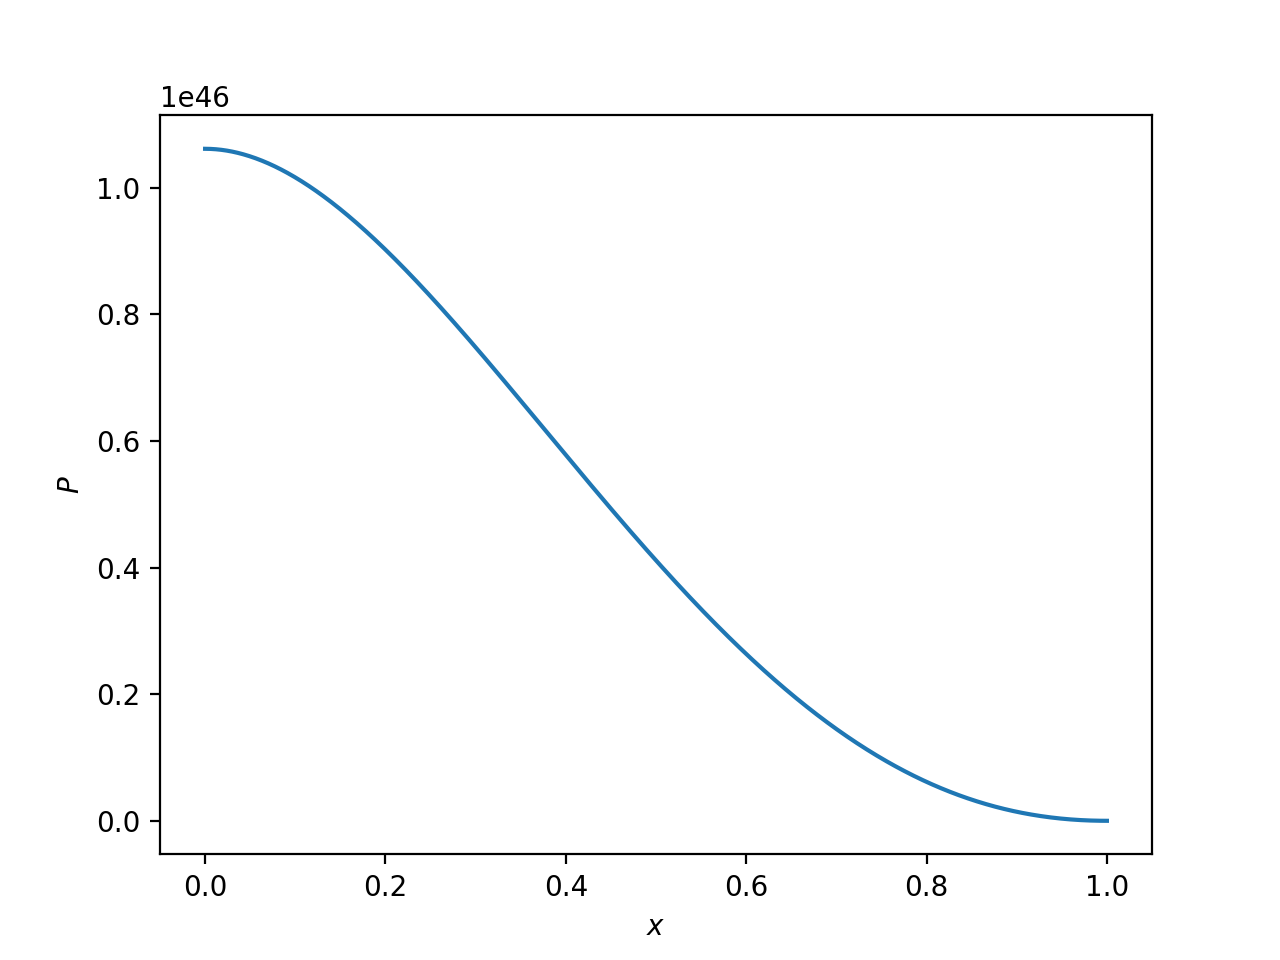
\includegraphics[width=15cm]{Figure_1.png}
    \caption{$P \; vs. \; x$.}
    \label{fig:img}
\end{figure}

\clearpage


\section*{Problem 4}

The Lane-Emden equation

$$
\frac{1}{\xi^{2}} \frac{d}{d\xi} \Bigg( \xi^{2} \frac{d \theta}{d \xi} \Bigg) = -\theta^{n}
$$

\subsection*{(a)}

The polytropic relation is gave as $P = K\rho^{\gamma}$ where $\gamma = 1/n + 1$. Therefore, it can now be expressed as

$$
P = K\rho^{(1 + 1/n)}
$$

since $\rho = \rho_{c} \theta^{n}$, this equation can also be expressed as 

$$
P = K\rho^{\gamma} \theta^{n \gamma}
$$

and replacing $\gamma$ again gives the equation 

\begin{align*}
P &= K\rho^{(1 + 1/n)} \theta^{n + 1} & \text{or} && P = P_{c} \theta^{n + 1}
\end{align*}

\subsection*{(b)}

When $n = 0$ the Lane-Emden equation is 

$$
\frac{1}{\xi^{2}} \frac{d}{d\xi} \Bigg( \xi^{2} \frac{d \theta}{d \xi} \Bigg) = -1
$$

The equation can be rewrote so that the equation can be integrated. The equation in integration form is

\begin{align*}
\xi^{2} \frac{d \theta}{d \xi} &= - \xi^{2} d \xi \\
&= - \int \xi^{2} d \xi \\
&= - \frac{\xi^{3}}{3} + c
\end{align*}

This equation can now be set up a second time to integrate, both $d\theta$ and $d\xi$. This equation in integration form is now

\begin{align*}
\int d \theta &= - \int \frac{\xi}{3} + \frac{c}{\xi^{3}} d\xi\\
\theta &= - \frac{\xi^{2}}{6} - \frac{c}{\xi} + d 
\end{align*}

here we have $c = 1$ and $d = 0$. Therefore,

$$
\theta &= 1 - \frac{\xi^{2}}{6}.
$$

When $\theta = 0$ at point $\xi = \xi_{1}$, then

\begin{align*}
1 - \frac{\xi_{1}^{2}}{6} &= 0 \\
\frac{\xi_{1}^{2}}{6}  &= 1 \\
\xi_{1}^{2} &= 6 \\
\xi_{1} &= \sqrt{6} \\
\end{align*}

\clearpage

\section*{Appendix}

\subsection*{}
\lstinputlisting{homework_2.py}

\clearpage


% -------------------------- EOD -------------------------- 
\end{document}